\section{Auswertung}
\label{sec:Auswertung}
In diesem Versuch wird Rohr 1 mit einem Innendurchmesser von $10 \, \unit{\milli\meter}$ und Rohr 2 mit einem Innendurchmesser von $16 \, \unit{\milli\meter}$
vermessen.
\subsection{Bestimmung der Strömungsgeschwindigkeit als Funktion des Dopplerwinkels}
Die zur Berechnung der Strömungsgeschwindigkeit aufgenommenen Messwerte, sind für Rohr 1 in Tabelle (\ref{tab:Messung1_Rohr1}) und für Rohr 2 in Tabelle 
(\ref{tab:Messung1_Rohr2}) aufgelistet. 

\begin{table}[H]
    \centering
    \caption{Pumpgeschwindigkeit $v_\text{Pumpe}$, Frequenzverschiebung $\Delta \nu$ und Prismenwinkel $\theta$ der Messung an Rohr 1.}
    \label{tab:Messung1_Rohr1}
    \begin{tblr}{colspec={c c c c}}
        \toprule
        $v_\text{Pumpe} \, \left[\unit[per-mode=fraction]{\liter\per\minute}\right]$ & $\Delta \nu \,\, \text{bei}\,\, \theta = 15° \, \left[\unit[per-mode=fraction]{\hertz}\right]$  & $\Delta \nu \,\, \text{bei}\,\, \theta = 30° \, \left[\unit[per-mode=fraction]{\hertz}\right]$  & $\Delta \nu \,\,\text{bei}\,\, \theta = 45° \, \left[\unit[per-mode=fraction]{\hertz}\right]$ \\
        \midrule
        3   & 146  & 244 & 426 \\
        3,5 & 183  & 281 & 531 \\
        4   & 220  & 360 & 617 \\
        4,5 & 256  & 470 & 781 \\
        5   & 281  & 488 & 916 \\ 
        \bottomrule
    \end{tblr}
\end{table}
\begin{table}[H]
    \centering
    \caption{Pumpgeschwindigkeit $v_\text{Pumpe}$, Frequenzverschiebung $\Delta \nu$ und Prismenwinkel $\theta$ der Messung an Rohr 2.}
    \label{tab:Messung1_Rohr2}
    \begin{tblr}{colspec={c c c c}}
        \toprule
        $v_\text{Pumpe} \, \left[\unit[per-mode=fraction]{\liter\per\minute}\right]$ & $\Delta \nu \,\, \text{bei}\,\, \theta = 15° \, \left[\unit[per-mode=fraction]{\hertz}\right]$  & $\Delta \nu \,\, \text{bei}\,\, \theta = 30° \, \left[\unit[per-mode=fraction]{\hertz}\right]$  & $\Delta \nu \,\,\text{bei}\,\, \theta = 45° \, \left[\unit[per-mode=fraction]{\hertz}\right]$ \\
        \midrule
        3   & 61   & 110 & 183 \\
        3,5 & 73   & 134 & 208 \\
        4   & 85   & 146 & 293 \\
        4,5 & 110  & 220 & 342 \\
        5   & 146  & 256 & 439 \\ 
        \bottomrule
    \end{tblr}
\end{table}
Aus diesen Werten wird mithilfe von Formel (\ref{eqn:Stroemungsgeschwindigkeit}) die Strömungsgeschwindigkeit $v$ bestimmt. 
Diese ist in Tabelle (\ref{tab:Stroemungsgeschwindigkeit1_rohr1}) für Rohr 1 und in Tabelle (\ref{tab:Stroemungsgeschwindigkeit1_rohr2}) für Rohr 2 vermerkt. 
\begin{table}[H]
    \centering
    \caption{Berechnete Strömungsgeschwindigkeit $v$ an Rohr 1 dargestellt nach verwendetem Prismenwinkel $\theta$.}
    \label{tab:Stroemungsgeschwindigkeit1_rohr1}
    \begin{tblr}{colspec={c c c}}
        \toprule
        $v \,\, \text{bei}\,\, \theta = 15° \, \left[\unit[per-mode=fraction]{\meter\per\second}\right]$ & $v \,\, \text{bei}\,\, \theta = 30° \, \left[\unit[per-mode=fraction]{\meter\per\second}\right]$  & $v \,\, \text{bei}\,\, \theta = 45° \, \left[\unit[per-mode=fraction]{\meter\per\second}\right]$ \\
        \midrule
        0,3808 & 0,3294 & 0,4067 \\
        0,4773 & 0,3794 & 0,5069 \\
        0,5738 & 0,4860 & 0,5890 \\
        0,6676 & 0,6345 & 0,7455 \\
        0,7328 & 0,6588 & 0,8744 \\
        \bottomrule
    \end{tblr}
\end{table}
\begin{table}[H]
    \centering
    \caption{Berechnete Strömungsgeschwindigkeit $v$ an Rohr 2 dargestellt nach verwendetem Prismenwinkel $\theta$.}
    \label{tab:Stroemungsgeschwindigkeit1_rohr2}
    \begin{tblr}{colspec={c c c}}
        \toprule
        $v \,\, \text{bei}\,\, \theta = 15° \, \left[\unit[per-mode=fraction]{\meter\per\second}\right]$ & $v \,\, \text{bei}\,\, \theta = 30° \, \left[\unit[per-mode=fraction]{\meter\per\second}\right]$  & $v \,\, \text{bei}\,\, \theta = 45° \, \left[\unit[per-mode=fraction]{\meter\per\second}\right]$ \\
        \midrule
        0,1591 & 0,1485 & 0,1747 \\
        0,1904 & 0,1809 & 0,1986 \\
        0,2217 & 0,1971 & 0,2797 \\
        0,2869 & 0,2970 & 0,3265 \\
        0,3808 & 0,3456 & 0,4191 \\
        \bottomrule
    \end{tblr}
\end{table}

Die Frequenzverschiebung geteilt durch $\cos(\alpha)$ wird in Abbildung (\ref{fig:Abschnitt1_10mm}) gegen die Strömungsgeschwindigkeit für Rohr 1 aufgetragen und 
in Abbildung (\ref{fig:Abschnitt1_16mm}) für Rohr 2. Die 
Frequenzverschiebung geteilt durch $\cos(\alpha)$ ist für Rohr 1 in Tabelle (\ref{tab:delta_geteilt_cosalpha_1}) aufgeführt unf für Rohr 2 in Tabelle (\ref{tab:delta_geteilt_cosalpha_2}). 
\begin{table}[H]
    \centering
    \caption{Pumpgeschwindigkeit $v_\text{Pumpe}$, Frequenzverschiebung $\frac{\Delta \nu}{\cos(\alpha)}$ und Prismenwinkel $\theta$ der Messung an Rohr 1.}
    \label{tab:delta_geteilt_cosalpha_1}
    \begin{tblr}{colspec={c c c c}}
        \toprule
        $v_\text{Pumpe} \, \left[\unit[per-mode=fraction]{\liter\per\minute}\right]$ & $\frac{\Delta \nu}{\cos(\alpha)} \,\, \text{bei}\,\, \theta = 15° \, \left[\unit[per-mode=fraction]{\hertz}\right]$  & $\frac{\Delta \nu}{\cos(\alpha)} \,\, \text{bei}\,\, \theta = 30° \, \left[\unit[per-mode=fraction]{\hertz}\right]$  & $\frac{\Delta \nu}{\cos(\alpha)} \,\,\text{bei}\,\, \theta = 45° \, \left[\unit[per-mode=fraction]{\hertz}\right]$ \\
        \midrule
        3   & 846  & 732  & 904 \\
        3,5 & 1060 & 843  & 1126 \\
        4   & 1275 & 1080 & 1309 \\
        4,5 & 1483 & 1410 & 1657 \\
        5   & 1628 & 1464 & 1943 \\ 
        \bottomrule
    \end{tblr}
\end{table}

\begin{table}[H]
    \centering
    \caption{Pumpgeschwindigkeit $v_\text{Pumpe}$, Frequenzverschiebung $\frac{\Delta \nu}{\cos(\alpha)}$ und Prismenwinkel $\theta$ der Messung an Rohr 2.}
    \label{tab:delta_geteilt_cosalpha_2}
    \begin{tblr}{colspec={c c c c}}
        \toprule
        $v_\text{Pumpe} \, \left[\unit[per-mode=fraction]{\liter\per\minute}\right]$ & $\frac{\Delta \nu}{\cos(\alpha)} \,\, \text{bei}\,\, \theta = 15° \, \left[\unit[per-mode=fraction]{\hertz}\right]$  & $\frac{\Delta \nu}{\cos(\alpha)} \,\, \text{bei}\,\, \theta = 30° \, \left[\unit[per-mode=fraction]{\hertz}\right]$  & $\frac{\Delta \nu}{\cos(\alpha)} \,\,\text{bei}\,\, \theta = 45° \, \left[\unit[per-mode=fraction]{\hertz}\right]$ \\
        \midrule
        3   & 354 & 330 & 388 \\
        3,5 & 423 & 402 & 441 \\
        4   & 493 & 438 & 622 \\
        4,5 & 638 & 660 & 725 \\
        5   & 846 & 768 & 931 \\ 
        \bottomrule
    \end{tblr}
\end{table}

\begin{figure}[H]
   \centering
   \caption{Frequenzverschiebung aufgetragen gegen die Strömunggeschwindigkeit mit Ausgleichsgerade für Rohr 1.}
   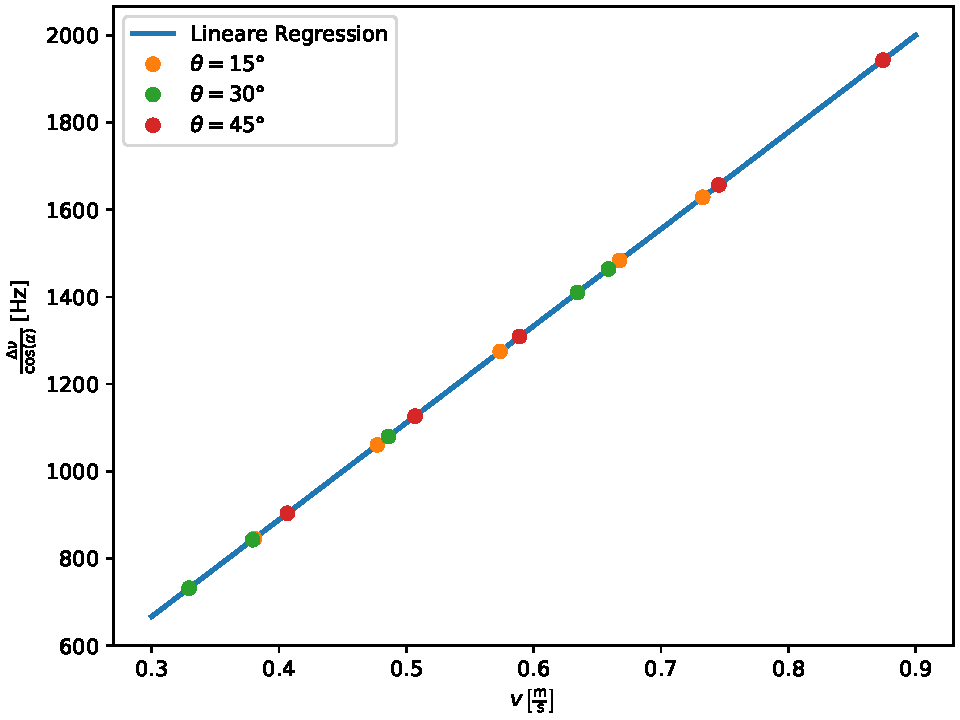
\includegraphics[width=0.8\linewidth]{plot1.pdf}
   \label{fig:Abschnitt1_10mm}
\end{figure}

\begin{figure}[H]
    \centering
    \caption{Frequenzverschiebung aufgetragen gegen die Strömunggeschwindigkeit mit Ausgleichsgerade für Rohr 2.}
    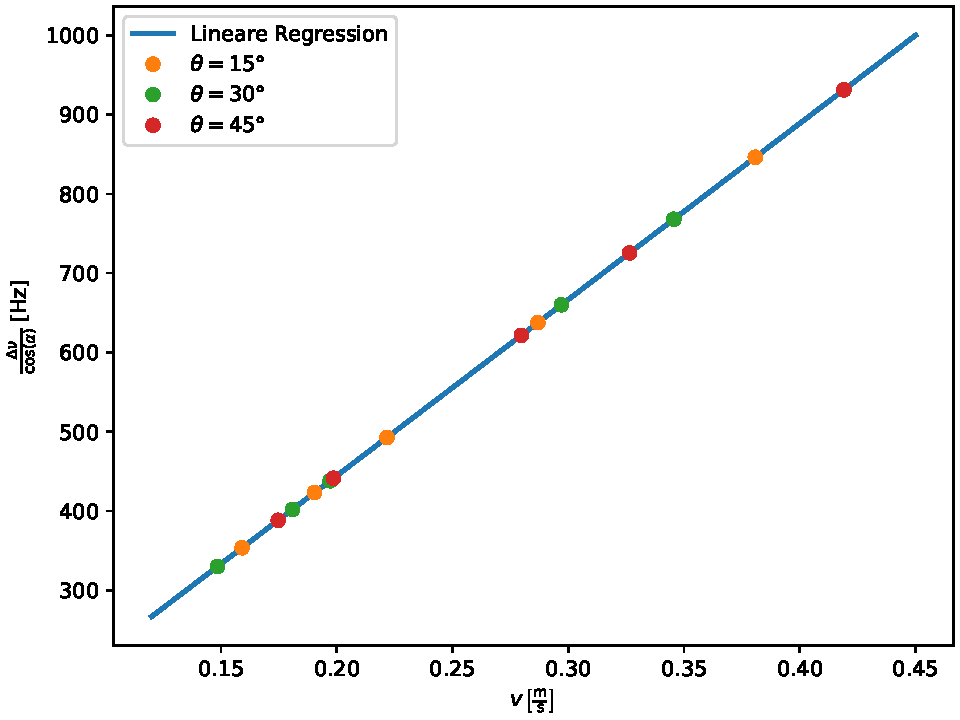
\includegraphics[width=0.8\linewidth]{plot2.pdf}
    \label{fig:Abschnitt1_16mm}
\end{figure}
Beide Ausgleichgeraden haben die Form $y = mx + n$. Für Rohr 1 ergibt sich dabei $m_1 = 2222,22 \, \unit[per-mode=fraction]{\per\meter}$ und $n_1 = 0 \, \unit{\hertz}$. Für Rohr 2 betragen die Werte 
ebenfalls  $m_2 = 2222,22 \, \unit[per-mode=fraction]{\per\meter}$ und $n_2 = 0 \, \unit{\hertz}$. 

Da die Messgrößen den linearen Zusammenhang $mv = \frac{\Delta \nu}{\cos(\alpha)}$ (für $n = 0$) haben, können die Unbekannten $x_1, x_2, x_3$ in den Formeln
\begin{align*}
    v_{15°} &= x_1 \cdot \Delta \nu \\
    v_{30°} &= x_2 \cdot \Delta \nu \\
    v_{45°} &= x_3 \cdot \Delta \nu \\
\end{align*}
zu 
\begin{align*}
    x_1 &= \frac{1}{m \cdot \cos(\alpha_{15°})} \approx 2,6080 \cdot 10^{-3}\, \unit{\meter}\\
    x_2 &= \frac{1}{m \cdot \cos(\alpha_{30°})} \approx 1,3501 \cdot 10^{-3}\, \unit{\meter}\\
    x_3 &= \frac{1}{m \cdot \cos(\alpha_{45°})} \approx 0,9545 \cdot 10^{-3}\, \unit{\meter}\\
\end{align*}
bestimmt werden. Aus der Formel (\ref{eqn:Stroemungsgeschwindigkeit}) lässt sich für den linearen Zusammenhang von $mv = \frac{\Delta \nu}{\cos(\alpha)}$ ein 
Theoriewert von $m_{\text{theo}} = \frac{2\nu_0}{c} \approx 2222,22 \, \unit[per-mode=fraction]{\per\meter}$ bestimmen.



\subsection{Bestimmung des Strömungsprofils der Dopplerflüssigkeit}
Zur Bestimmung des Strömungsprofils in Rohr 1 und Rohr 2 wird zu verschiedenen Tiefen die Frequenzverschiebung bei einem Prismawinkel von $15°$ gemessen. 
Dies wird bei einer Pumpgeschwindigkeit von $3 \, \unit[per-mode=fraction]{\liter\per\minute}$ und $6 \, \unit[per-mode=fraction]{\liter\per\minute}$ durchgeführt. 
Die Messdaten von Rohr 1 sind in Tabelle(\ref{tab:Messdaten_2_Rohr1}) und zu Rohr 2 in Tabelle (\ref{tab:Messdaten_2_Rohr2}) aufgelistet. 

\begin{table}[H]
    \centering
    \caption{Gemessenen Frequenzverschiebung $\Delta\nu_3$ und $\Delta\nu_6$ zu Messtiefe $x$ bei Pumpgeschwindigkeit $v_{\text{Pumpe}} = 3 \, \unit[per-mode=fraction]{\liter\per\minute}$ und $v_{\text{Pumpe}} = 6 \, \unit[per-mode=fraction]{\liter\per\minute}$ in Rohr 1.}
    \label{tab:Messdaten_2_Rohr1}
    \begin{tblr}{colspec={c c c}}
        \toprule
        $x \, \left[\unit[per-mode=fraction]{\micro\second}\right]$ & $\Delta\nu_3 \,  \left[\unit[per-mode=fraction]{\hertz}\right]$  &  $\Delta\nu_6 \,  \left[\unit[per-mode=fraction]{\hertz}\right]$\\
        \midrule
        12      & 0       & 0   \\
        12,5    & 0       & 281 \\
        13      & 0       & 342 \\
        13,5    & 146     & 391 \\
        14      & 159     & 464 \\
        14,5    & 171     & 525 \\
        15      & 183     & 580 \\
        15,5    & 183     & 574 \\
        16      & 171     & 513 \\
        16,5    & 159     & 431 \\
        17      & 144     & 342 \\
        17,5    & 122     & 293 \\
        18      & 122     & 269 \\
        \bottomrule
    \end{tblr}
\end{table}

\begin{table}[H]
    \centering
    \caption{Gemessenen Frequenzverschiebung $\Delta\nu_3$ und $\Delta\nu_6$ zu Messtiefe $x$ bei Pumpgeschwindigkeit $v_{\text{Pumpe}} = 3 \, \unit[per-mode=fraction]{\liter\per\minute}$ und $v_{\text{Pumpe}} = 6 \, \unit[per-mode=fraction]{\liter\per\minute}$ in Rohr 2.}
    \label{tab:Messdaten_2_Rohr2}
    \begin{tblr}{colspec={c c c}}
        \toprule
        $x \, \left[\unit[per-mode=fraction]{\micro\second}\right]$ & $\Delta\nu_3 \,  \left[\unit[per-mode=fraction]{\hertz}\right]$  &  $\Delta\nu_6 \,  \left[\unit[per-mode=fraction]{\hertz}\right]$\\
        \midrule
        12      & 0       & 0   \\
        12,5    & 0       & 0   \\
        13      & 0       & 0   \\
        13,5    & 0       & 0   \\
        14      & 0       & 171 \\
        14,5    & 0       & 195 \\
        15      & 73      & 232 \\
        15,5    & 85      & 269 \\
        16      & 85      & 305 \\
        16,5    & 85      & 317 \\
        17      & 85      & 332 \\
        17,5    & 85      & 293 \\
        18      & 79      & 269 \\
        18,5    & 73      & 269 \\
        19      & 73      & 244 \\
        \bottomrule
    \end{tblr}
\end{table}
Aus diesen Daten werden für beide Rohre und beide Pumpgeschwindigkeiten die Momentangeschwindigkeiten mithilfe von Formel (\ref{eqn:Stroemungsgeschwindigkeit})
berechnen. Die berechneten Momentangeschwindigkeiten sind in Tabelle (\ref{tab:Momentangeschwindigkeiten_1}) für Rohr 1 und in Tabelle (\ref{tab:Momentangeschwindigkeiten_2})
für Rohr 2 zu finden. 
\begin{table}[H]
    \centering
    \caption{Momentangeschwindigkeiten $v$ nach Pumpgeschwindigkeit unterschieden für Rohr 1.}
    \label{tab:Momentangeschwindigkeiten_1}
    \begin{tblr}{colspec={c c}}
        \toprule
        $v \,\, \text{bei} \,\, v_{\text{Pumpe}} =  3 \, \unit[per-mode=fraction]{\liter\per\minute}\, \left[\unit[per-mode=fraction]{\meter\per\second}\right]$ & $v \,\, \text{bei} \,\, v_{\text{Pumpe}} =  6 \, \unit[per-mode=fraction]{\liter\per\minute}\, \left[\unit[per-mode=fraction]{\meter\per\second}\right]$ \\
        \midrule
        0          & 0          \\
        0          & 0,7328     \\
        0          & 0,8919     \\
        0,3808     & 1,0197     \\
        0,4147     & 1,2101     \\
        0,4460     & 1,3692     \\
        0,4773     & 1,5126     \\
        0,4773     & 1,4970     \\
        0,4460     & 1,3379     \\
        0,4147     & 1,1240     \\
        0,3756     & 0,8919     \\
        0,3182     & 0,7641     \\
        0,3182     & 0,7016     \\
        \bottomrule
    \end{tblr}
\end{table}

\begin{table}[H]
    \centering
    \caption{Momentangeschwindigkeiten $v$ nach Pumpgeschwindigkeit unterschieden für Rohr 2.}
    \label{tab:Momentangeschwindigkeiten_2}
    \begin{tblr}{colspec={c c}}
        \toprule
        $v \,\, \text{bei} \,\, v_{\text{Pumpe}} =  3 \, \unit[per-mode=fraction]{\liter\per\minute}\, \left[\unit[per-mode=fraction]{\meter\per\second}\right]$ & $v \,\, \text{bei} \,\, v_{\text{Pumpe}} =  6 \, \unit[per-mode=fraction]{\liter\per\minute}\, \left[\unit[per-mode=fraction]{\meter\per\second}\right]$ \\
        \midrule
        0           & 0          \\          
        0           & 0          \\          
        0           & 0          \\          
        0           & 0          \\  
        0           & 0,4460     \\  
        0           & 0,5086     \\ 
        0,1904      & 0,6051     \\  
        0,2217      & 0,7016     \\  
        0,2217      & 0,7954     \\  
        0,2217      & 0,8267     \\  
        0,2217      & 0,8659     \\  
        0,2217      & 0,7641     \\ 
        0,2060      & 0,7016     \\
        0,1904      & 0,7016     \\
        0,1904      & 0,6364     \\ 
        \bottomrule
    \end{tblr}
\end{table}
Diese Momentangeschwindigkeiten werden gegen die Messtiefe $x$ für Rohr 1 in Abbildung (\ref{fig:Momentan_1}) und für Rohr 2 in Abbildung (\ref{fig:Momentan_2})
aufgetragen. 
\begin{figure}[H]
    \centering
    \caption{Momentangeschwindigkeit aufgetragen gegen die Messtiefe für Rohr 1.}
    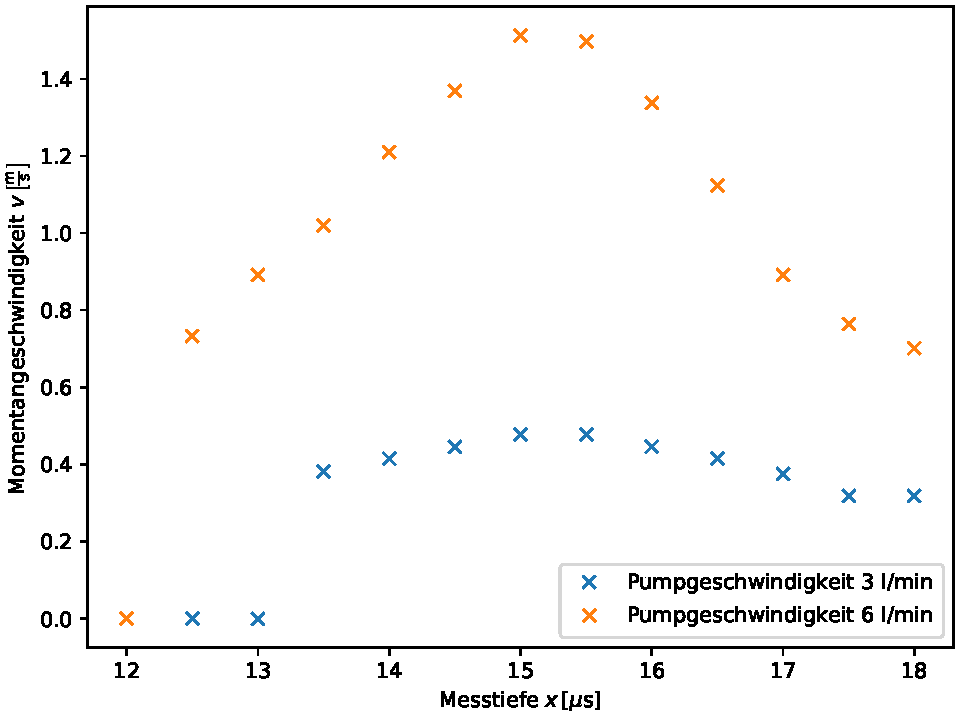
\includegraphics[width=0.82\linewidth]{plot3.pdf}
    \label{fig:Momentan_1}
\end{figure}
\begin{figure}[H]
    \centering
    \caption{Momentangeschwindigkeit aufgetragen gegen die Messtiefe für Rohr 2.}
    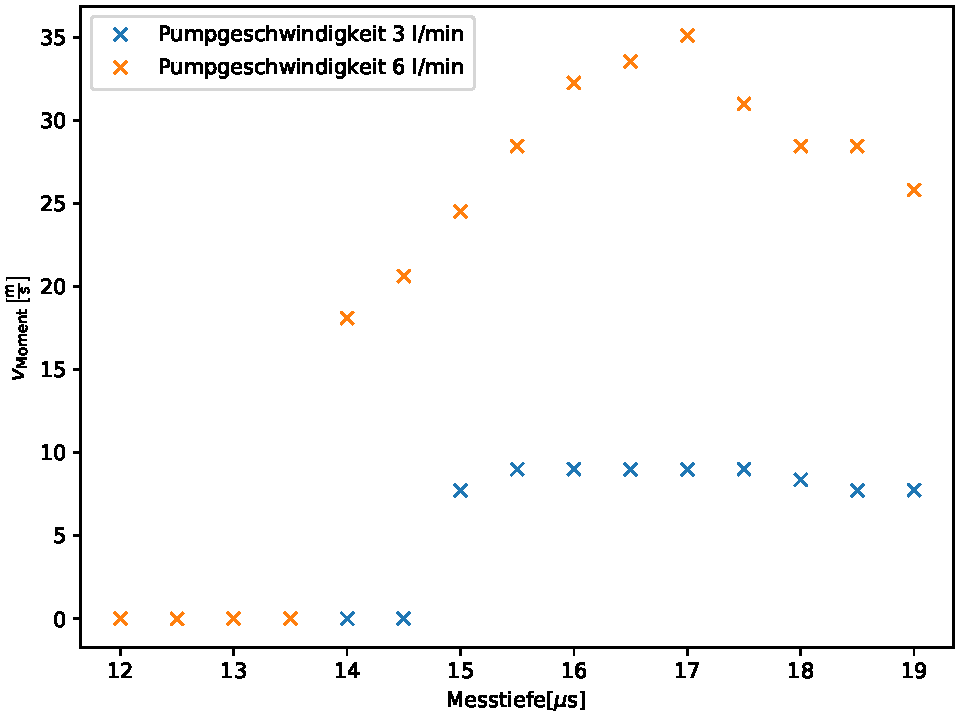
\includegraphics[width=0.82\linewidth]{plot4.pdf}
    \label{fig:Momentan_2}
\end{figure}
                                            
%Siehe \autoref{fig:plot}!